\begin{frame}{The Standard Model of Particle Physics}
  \framesubtitle{State of the art}

  \begin{columns}
    
    \begin{column}{0.5\textwidth}

      \begin{figure}
        \centering
        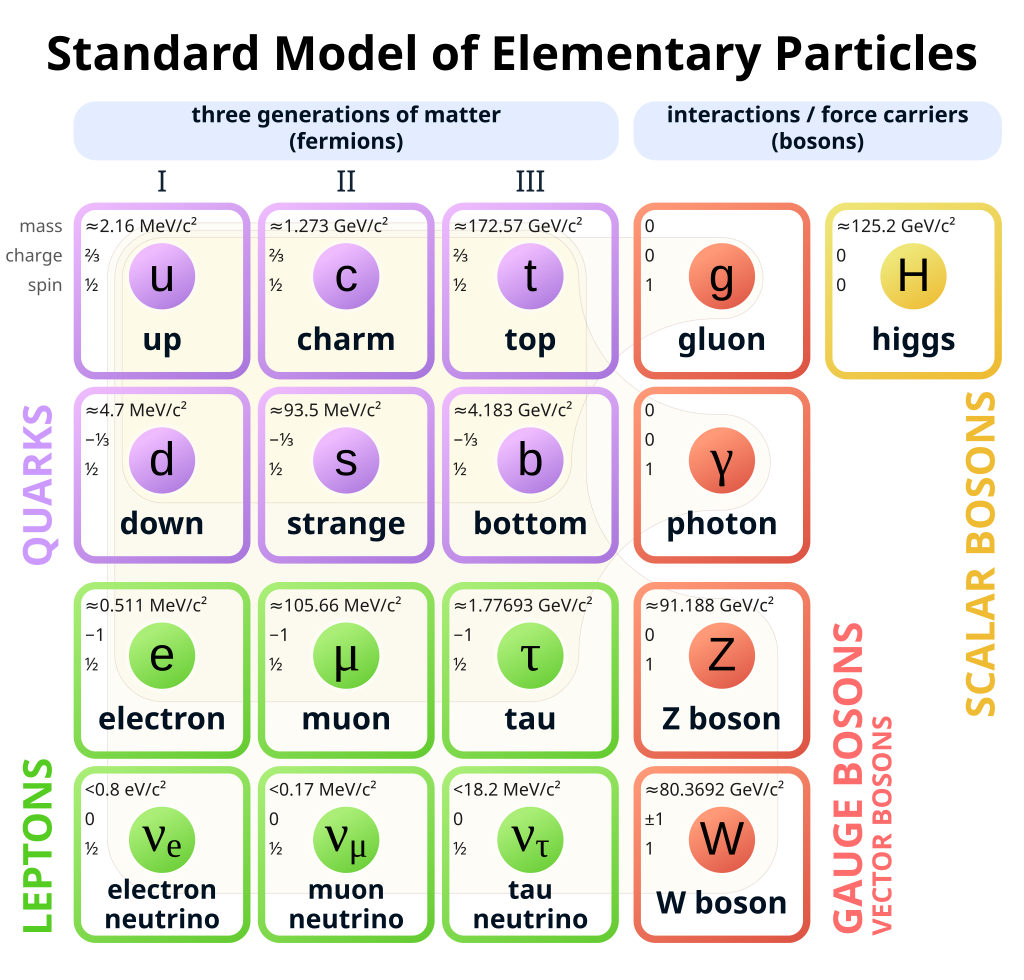
\includegraphics[width = \textwidth]{imgs/standard-model.png}
      \end{figure}

    \end{column}

    

    \begin{column}{0.5 \textwidth}
    \begin{center}
        High energy $\to$ Special Relativity \\
        Small particles $\to$ Quantum Mechanics \\
        $\downarrow$ \\
        Quantum Field Theory \\
        (mathematical framework)
    \end{center}
    
    

      \begin{colorblock}[black]{statalelightgreen}{Evidences for physics beyond the SM}
        \begin{itemize}
          \item Dark matter and dark energy
          \item Matter-antimatter asymmetry
          \item Origin of neutrino masses
        \end{itemize}
      \end{colorblock}

      \vspace{0.5em}


      

    \end{column}

  \end{columns}

\end{frame}

%=======================================================================

\begin{frame} {Collider Physics}
  \framesubtitle{One of the principal methods of research}

   \begin{columns}
  
    \begin{column}{0.5\textwidth}
    \textbf{L}arge \textbf{H}adron \textbf{C}ollider at CERN \\
    Proton beams accelerated to $\sim 13.6 \, \text{TeV}$ \\

      \begin{figure}
        \centering
        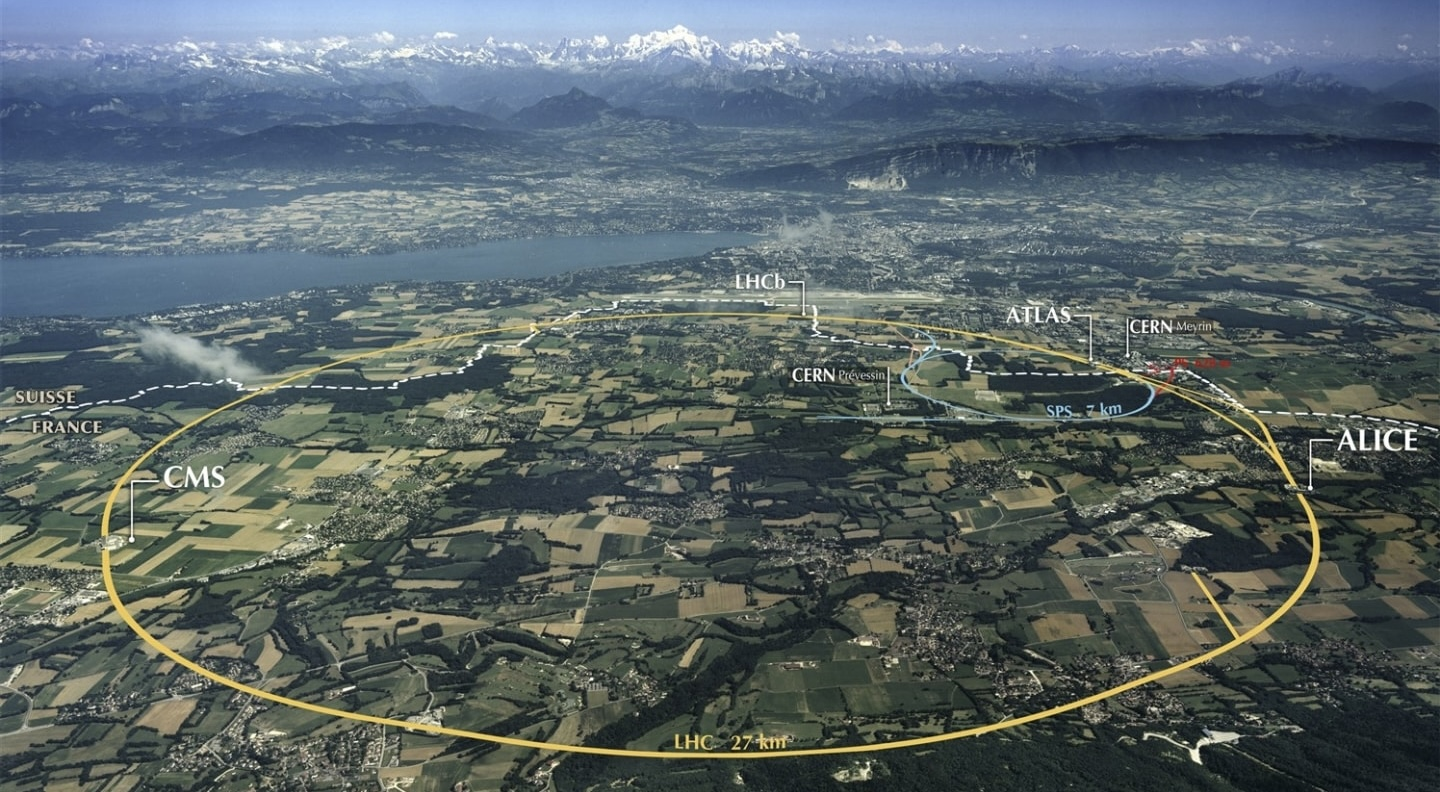
\includegraphics[width=\textwidth]{imgs/lhc.jpeg}
        \caption{ Maximilien Brice/CERN}
      \end{figure}
    \end{column}


    \begin{column}{0.5\textwidth}
        \begin{centering}
            Not sufficient to the discovery of new particles. \\

            \vspace{2.0em}
        Solutions: 
        \vspace{0.8em}
        \begin{itemize}
        \item Increase energy \\$\to$ not feasible with existing technology
        \end{itemize}
        \end{centering}

        \begin{colorblock}[black]{statalelightgreen}{}
        \begin{itemize}
          \item Increase precision  \\$\to$ both experimental and \textbf{theoretical}
        \end{itemize}
      \end{colorblock}
    
    \end{column}

    \end{columns}
  
\end{frame}


%=======================================================================

\begin{frame} {Quantum Chromodynamics}
  \framesubtitle{Hard scattering processes}

   \begin{columns}

    \begin{column}{0.5\textwidth}

    \vspace{0.5em}
    
        \begin{itemize}
            \item Strong interactions are described by Quantum Chromodynamics (QCD).
            \item Non-Abelian gauge theory, \\$SU(3)$ symmetry group.
            \item The QCD Lagrangian is not analytically solvable.
        \end{itemize}

    \vspace{0.5em}
    \begin{colorblock}[black]{statalelightgreen}{Hadron collisions}
        \begin{itemize}
          \item Elastic scattering
          \item Diffractive dissociation
          \item Hard scattering \\(momentum exchange $\sim 100 \,\text{GeV}$)
        \end{itemize}
      \end{colorblock}
    
  
    \end{column}

    \begin{column}{0.5\textwidth}
        \begin{figure}
        \centering
        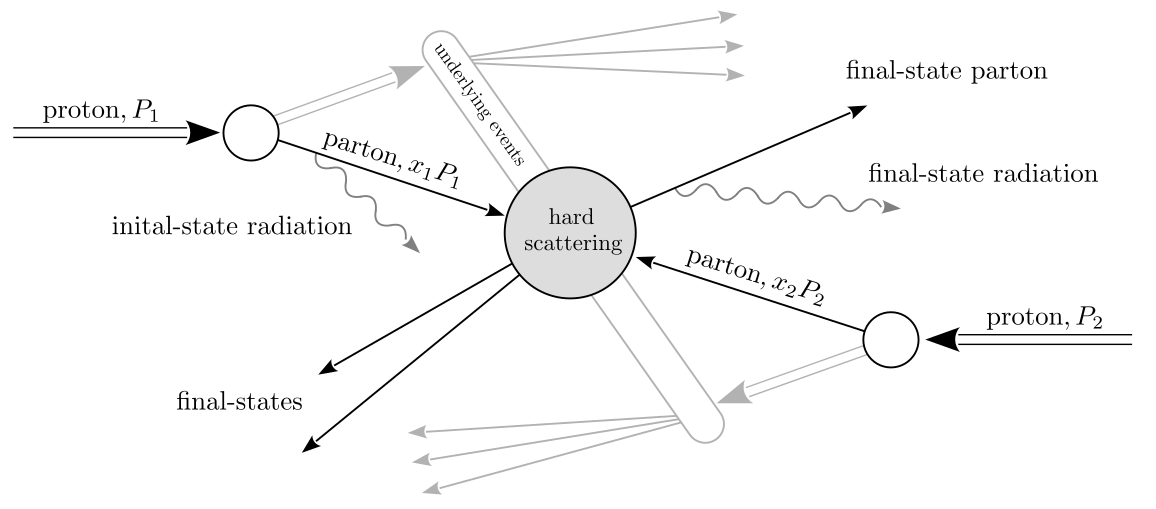
\includegraphics[width=\textwidth]{imgs/hard-scattering.png}
        \caption{Konstantin Asteriadis/KIT}
      \end{figure}

      \textbf{Asymptotic freedom} \\
      Interacting partons can be approximated as being nearly free\\
      $\to$ \textbf{Perturbative description}
    
    \end{column}

    \end{columns}
  
\end{frame}


%=======================================================================

\begin{frame} {The collinear factorization theorem}
  \framesubtitle{A framework for describing hard scattering processes}
    
   \begin{columns}

    \begin{column}{0.6\textwidth}
    Colliding hadrons are treated as \textbf{beams of partons}, carrying a fraction of the hadron's total momentum
    
   \begin{colorblock}[black]{statalelightgreen}{Separation of energy scales}
        \begin{itemize}
          \item SM interactions $Q \sim 100 \text{GeV}-1\text{TeV}$
          \item Hadronic structure $\Lambda_{\mathrm{QCD}}\sim 100\text{MeV}$
        \end{itemize}
      \end{colorblock}
\begin{centering}
    $\to$ \textbf{Decoupling} the motions of partons from proton's dynamics
\end{centering}
    
    \end{column}

    \begin{column}{0.4\textwidth}
       \begin{figure}
        \centering
        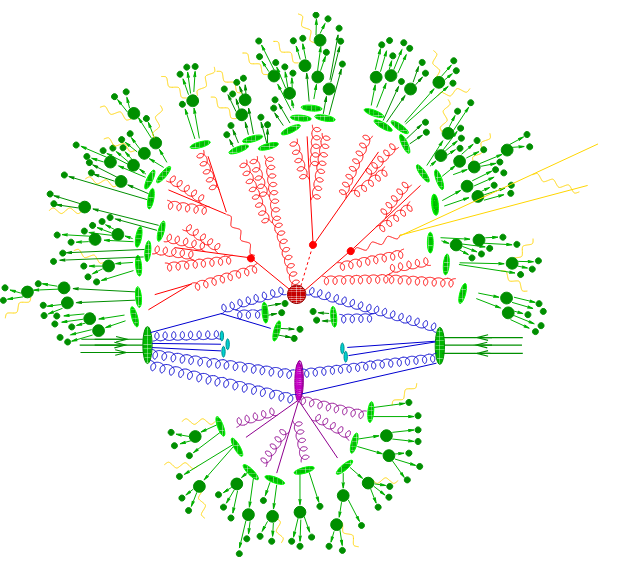
\includegraphics[width=0.8\textwidth]{imgs/hadron-collision.png}
        \caption{Stefan Höche/SLAC National Accelerator Laboratory}
      \end{figure}
    
    \end{column}

    \end{columns}
    \begin{equation*}
    \text{d}\sigma=\sum_{a, b} \int_0^1 \text{d}x_1 \text{d}x_2 f_{a}(x_1, \mu_\text{F}) f_{b}(x_2,\mu_\text{F}) \, \text{d}\hat \sigma_{a,b}(x_1,x_2,\mu_\text{F},\mu_\text{R};\mathcal{O}) \left(1+ \mathcal{O}\left(\frac{\Lambda_{\text{QCD}}}{Q} \right)^n \right), \, n\geq1
    \label{fact-theor}
\end{equation*}
  
\end{frame}


%=======================================================================

\begin{frame} {The partonic cross section}
  \framesubtitle{A perturbative description}
\vspace{1em}
The partonic cross section can be expanded in powers of the strong and the electroweak coupling constants, $\alpha_{\text{S}}$ and $\alpha$
    \begin{equation*}
    \text{d} \hat{\sigma}_{a,b} = \text{d} \hat{\sigma}_{a,b}^{(0,0)} + \textcolor{red}{\alpha_s \text{d} \hat{\sigma}_{a,b}^{(1,0)}} + \alpha_s^2 \text{d} \hat{\sigma}_{a,b}^{(2,0)} + \alpha_s^3 \text{d} \hat{\sigma}_{a,b}^{(3,0)} + \alpha \text{d} \hat{\sigma}_{a,b}^{(0,1)} + \alpha \alpha_s \text{d} \hat{\sigma}_{a,b}^{(1,1)} + \dots 
    \end{equation*}

    \begin{columns}

    \begin{column}{0.6\textwidth}
    \begin{colorblock}[black]{statalelightgreen}{We focus on  NLO QCD corrections}
    \begin{center}
        Account for short distance, high-energy effects
    \end{center}
      \end{colorblock}   
    
    \end{column}

    \begin{column}{0.4\textwidth}
    \\
    They consist of three terms 
    \begin{equation*}
    \textcolor{red}{\mathrm{d} \hat{\sigma}_{a,b}^{\mathrm{NLO}}} = \mathrm{d} \hat{\sigma}_{a,b}^{\mathrm{R}} + \mathrm{d} \hat{\sigma}_{a,b}^{\mathrm{V}} + \mathrm{d} \hat{\sigma}_{a,b}^{\mathrm{pdf}}
    \end{equation*}       
    
    \end{column}

    \end{columns}
    \begin{figure}
        \centering
        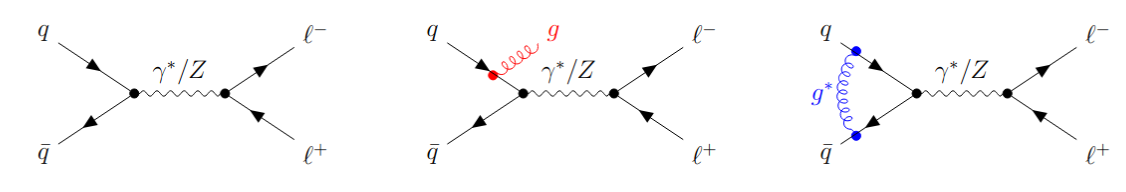
\includegraphics[width=0.8\textwidth]{imgs/real-and-virtual.png}
      \end{figure}    
\end{frame}


%=======================================================================

\begin{frame} {UV and IR divergences}
  \framesubtitle{A considerable obstacle}
  \vspace{1em}
  The treatment of real and virtual corrections is \textbf{non-trivial} \\
  \vspace{1em}
  \textcolor{maincolor}{\textcircled{1}} \textbf{Ultraviolet} (UV) singularities in virtual contributions \\
  \quad $\to$ Renormalization

    \begin{colorblock}[black]{statalelightgreen}{}
        \textcolor{maincolor}{\textcircled{2}} \textbf{Infrared} (IR) singularities in both real and virtual contributions \\
    \quad $\to$ Low-momentum (\textcolor{red}{soft}) and small-angle (\textcolor{blue}{collinear}) kinematic regions
      \end{colorblock}
    
\begin{equation*}
  \begin{tikzpicture}[baseline = (r.base)]
    \begin{feynman}[inline = (r.base)]
      \vertex (a);
      \vertex[right = 2cm of a, dot] (b) {};
      \vertex[right = 2cm of b, circle, draw, fill=lightgray,  minimum size = 1.2cm] (c) {};

      \vertex[above = 1cm of b] (d);
      \vertex[right = 1.5cm of d] (e);

      \vertex[below = 0.25cm of b] (r);

      \diagram* {
	    (a) -- [fermion, momentum' = \(p_i\)] (b),
	    (b) -- [fermion, momentum' = \(p_i - p_\um\)] (c),

	    (b) -- [gluon, momentum = \(p_\um\)] (e),
        };
    \end{feynman}
  \end{tikzpicture}
  \, \sim \,
  \frac{1}{(p_i - p_\um)^2} = \frac{1}{2 E_i E_\um \left( 1 - \cos \theta_{i \um} \right)} \quad
  \xrightarrow[\textcolor{red}{E_\um}, \textcolor{blue}{\theta_{i \um}} \to 0 ]{} \quad \infty \,
\end{equation*}

\end{frame}


%=======================================================================

\begin{frame} {UV and IR divergences}
  \framesubtitle{Dimensional regularization and pole cancellation}

  \begin{columns}

    \begin{column}{0.5\textwidth}
    \begin{colorblock}[black]{statalelightgreen}{Dimensional regularization}
        \begin{equation*}
            d=4-2\epsilon \qquad \epsilon \in \mathbb{C} \, , \mathrm{Re}(\epsilon)<0
        \end{equation*}
      \end{colorblock}
    \end{column}

    \begin{column}{0.5\textwidth}
    Divergences appear as poles in $1/\epsilon$ \\
    \begin{itemize}
        \item Virtual $\to$ explicit
        \item Real $\to$ integration needed \textcolor{red}{\textcircled{1}}
    \end{itemize}
    \end{column}
    \end{columns}

    \vspace{1.5em}

    \begin{itemize}
        \item Singularities signal the presence of \textbf{non-perturbative contributions}
        \item We lack methods to treat non-perturbative QCD effects from first principles
    \end{itemize}

    \vspace{1.em}

    \begin{colorblock}[black]{statalelightgreen}{Bloch-Nordsieck and Kinoshita-Lee-Nauenberg theorems}
            Infrared divergences are \textbf{guaranteed} to cancel when we sum real and virtual corrections
      \end{colorblock}

      \begin{itemize}
        \item \textbf{Mismatch} in the dimensionality of the integration domains \textcolor{red}{\textcircled{2}}
    \end{itemize}
\end{frame}

%=======================================================================

\begin{frame} {IR divergences}
 \framesubtitle{Subtraction scheme}
Insights \\
\begin{itemize}
    \item \textbf{Factorization} of the amplitudes in the soft and collinear limits 
    \item Real emissions are \textbf{unresolved} in singular kinematics regions
\end{itemize}
 \vspace{1.em}
 We adopt a \textbf{subtraction method}
\begin{equation*}
    2s_{a,b} \mathrm{d} \hat{\sigma}_{a,b}^{\mathrm{R}} = \int [\mathrm{d}p_{\um}] F_{\mathrm{LM}} (\um)=  \textcolor{red}{\int [\mathrm{d}p_{\um}] (F_{\mathrm{LM}}(\um) - \mathcal{S})}  + \textcolor{blue}{\int [\mathrm{d}p_{\um}] \mathcal{S}}
    \label{subtraction-flm}
\end{equation*}
\textcolor{blue}{$\to$} Describes the singular behaviour of the amplitude\\ 
\textcolor{red}{$\to$} Singular behaviour removed: numerical integration with Monte Carlo methods \\


\begin{colorblock}[black]{statalelightgreen}{}
\begin{center}
    Restricting the integration region to the \textbf{minimal necessary volume} is crucial for improving the efficiency of the computation
\end{center}
            
      \end{colorblock}


\end{frame}

